\documentclass{report}
% Many important packages
\usepackage{amsmath, amssymb, tcolorbox, logicproof, fancyhdr,
    enumitem, float, graphicx, amsthm, listings, xcolor, hyperref, cochineal, nicematrix, 
titlesec, tcolorbox, tikz, pgfplots}
\hypersetup{hidelinks}

\title{CS215 Assignment 1 Solutions }
\author{Satyam Sinoliya, 23B0958 \\ Vaibhav Singh, 23B1068 \\ Shaik Awez Mehtab, 23B1080}
\date{August 2024}

% Setting up the look of the page
\RequirePackage[a4paper,width=150mm,top=25mm,bottom=25mm]{geometry}

% To be able to write the code
\lstset { %
	language=C++,
	basicstyle=\fontfamily{pcr}\footnotesize,
	keepspaces=true,
}

% For breakable tcolorbox
\tcbuselibrary{listings,breakable}

% No need to include whole path everytime
\graphicspath{{./images/}}

% For drawing graph in q4
\pgfplotsset{compat=1.18}
\usepgfplotslibrary{fillbetween}

\theoremstyle{definition}
\newtheorem{sol}{Solution} % Use this for writing solutions
\newtheorem{que}{Question} % For questions
\newtheorem{theorem}{Theorem} % For theorems
\newtheorem{lemma}{Lemma} % For lemmas
\newtheorem{corollary}{Corollary} % For corollaries

\renewcommand{\complement}{\mathsf{c}}
\newcommand{\C}[2]{^{#1}C_{#2}}

\fancypagestyle{myfooter}{
    \fancyhf{} 
    \fancyhead[L]{\textbf{CS215 Assignment 1}} % Text above the line
    \fancyhead[C]{}
    \fancyhead[R]{}
    \renewcommand{\headrulewidth}{0.4pt}

    \fancyfoot[L]{Awez}
    \fancyfoot[C]{Vaibhav}
    \fancyfoot[R]{Satyam}
    \renewcommand{\footrulewidth}{0.4pt}
}

% For Background Image
\usepackage{eso-pic}
\newcommand\BackgroundPic{%
\put(0,0){%
\parbox[b][\paperheight]{\paperwidth}{%
\vfill
\centering
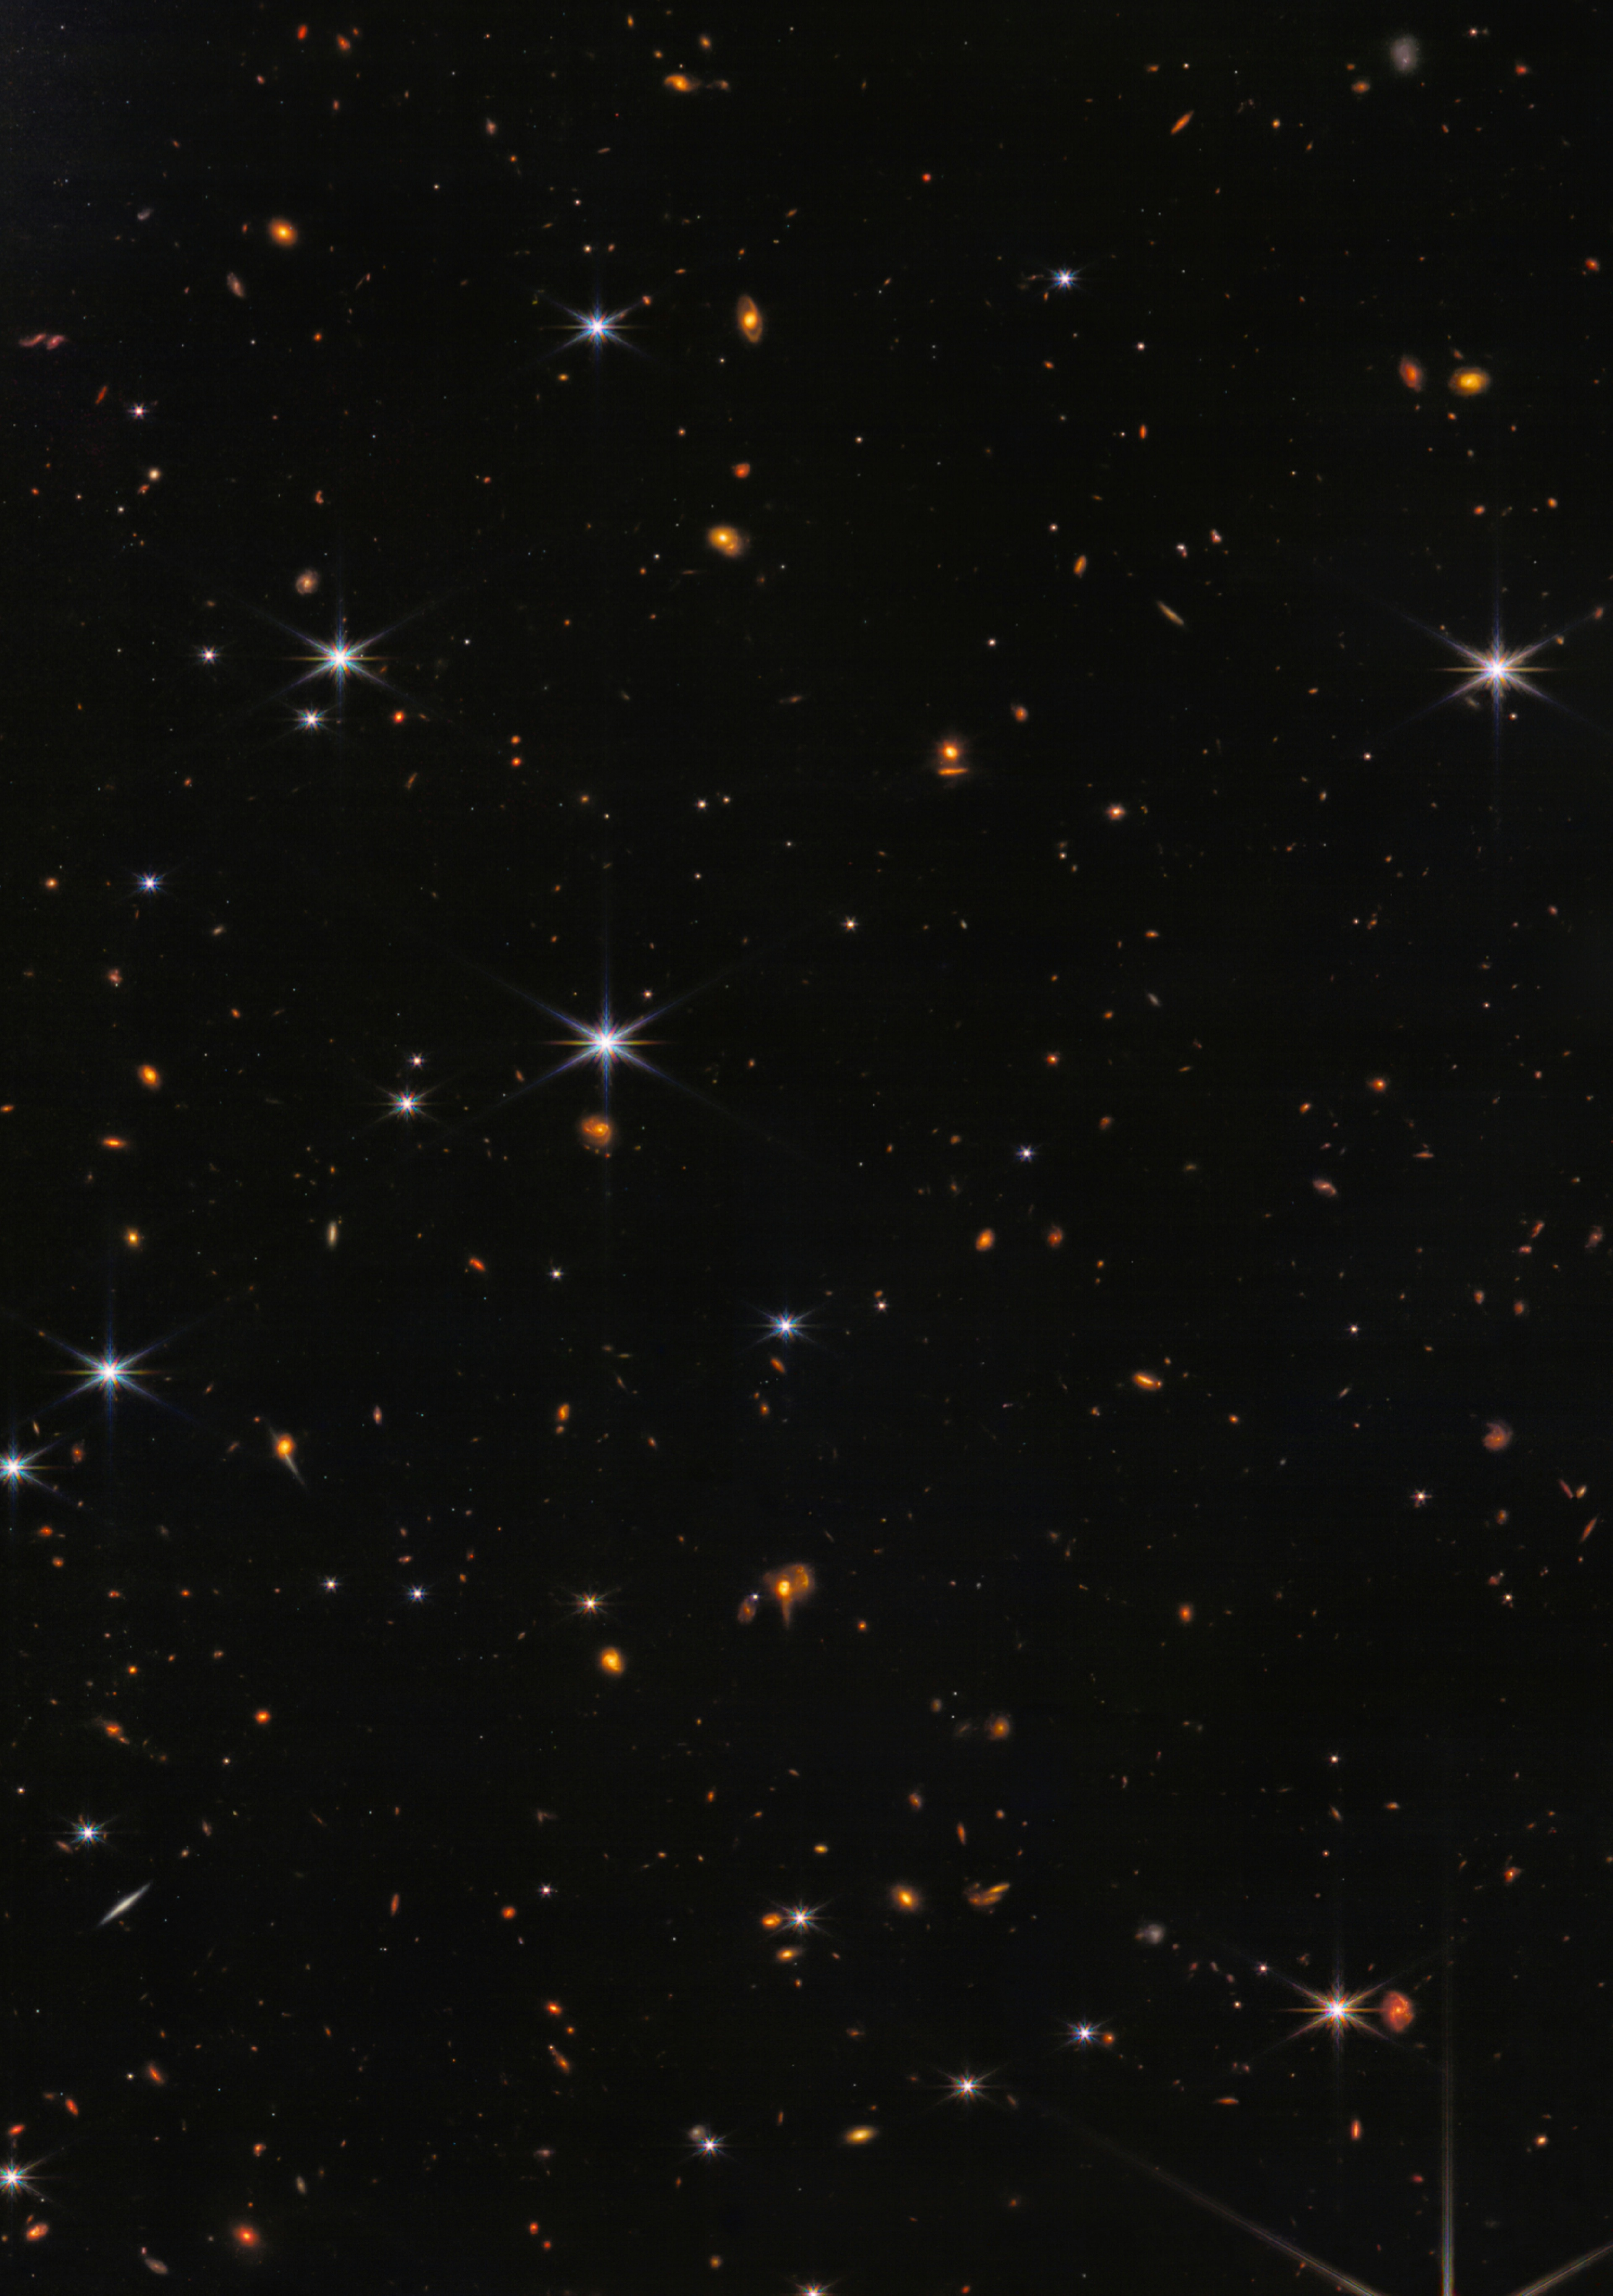
\includegraphics[width=\paperwidth,height=\paperheight,%
keepaspectratio]{images/bg.jpg}%
\vfill
}}}

\pagestyle{myfooter}

\begin{document}

\color{white}
\AddToShipoutPicture*{\BackgroundPic}
\maketitle
\color{black}

\section{Parking lot problem}
\subsection{Part a)}
The MAPE and MASE of the model for the testing dataset is as follows:
\begin{itemize}[noitemsep]
	\item MAPE:  5.349685330136059
	\item MASE:  0.6598538430731961
\end{itemize}


\subsection{Part b)}
The MAPE and MASE of the model for the testing dataset is as follows:
\begin{itemize}[noitemsep]
	\item MAPE:  9.81429557710239
	\item MASE:  0.26311286911247267
\end{itemize}

\subsection{Part c)}
We have used the following smoothing techniques and the following results are achieved:
\begin{itemize}
	\item MAPE:  3.2338475891165857
	\item MASE:  0.17231581778569224
\end{itemize}

\begin{solution}
	% Fill you solution here
	\tcbsubtitle{Task A}
	\textbf{To prove: }\\
	\emph{Let $X$ be a continuous real-valued random variable with CDF  : $\mathbb{R} \rightarrow [0, 1]$. Assume that
	$F_X$ is invertible. Then the random variable $Y := F_X (X) \in [0, 1]$ is uniformly distributed in $[0, 1]$}\\
	\textbf{Proof:}\\
	$F_X$ by definition can also be written as
	\[F_X(x) = P(X\leq x)\]
	Define a new random variable $Y$,
	\[Y =F_X(X) \]
	Y is the result of applying CDF $F_X$ to the random variable $X$.
	To prove the theorem, assume $y\in [0,1]$. So, the probablity that $Y \leq y$ is:
	\[P(Y\leq y) = P(F_X(X)\leq y)\]
	It is assumed that $F_X(x)$ is invertible, so,
	\[P(Y\leq y) = P(X\leq F_X^{-1}(y))\]
	which is basically, probablity that $X$ is less that or equal to $F_X^{-1}(y)$. This can be written in the CDF form, which is $F_X(F_X^{-1}(y))$. So,
	\[P(Y\leq y) = P(X\leq F_X^{-1}(y)) = F_X(F_X^{-1}(y)) = y\]
	So,
	\[P(Y\leq y) = y\]
	where $y\in [0,1]$, which is the CDF of uniform distributon in $[0,1]$.
	So, Y is a uniform distributon in $[0,1]$ regardless of $X$.

	
\end{solution}

% Start writing your answer from here, if you want to use new packages/change something do it in main.tex
\begin{que}
		\textbf{3.1} Let $Q_{1}$, $Q_{2}$ be non-negative random variables. Let $P(Q_1 < q_1) \geq 1-p_1$ and $P(Q_2 < q_2) \geq 1-p_2$
		where $q_1, q_2$ are non-negative. Then show that $P(Q_1Q_2 < q_1q_2) \geq 1 - (p_1 + p_2)$\\
		\textbf{3.2} Given n distinct values ${\{x_i\}}^n_{i=1}$ with mean $\mu$ and standard deviation $\sigma$, prove that for all $i$,
		we have $|x_i - \mu| \leq \sigma \sqrt[]{n-1}$. How does this inequality compare with Chebyshev's inequality as n
		increases? (give an informal answer)
	

	\hspace*{\fill} [5 marks]
\end{que}

\begin{tcolorbox}[breakable]
	\begin{sol}
		\textbf{3.1}Define two events, $E_1$ and $E_2$:
		\begin{enumerate}
			\item $E_1=\{Q_1<q_1\}$
			\item $E_2=\{Q_2<q_2\}$
		\end{enumerate}
		So,
		\[P(E_1)\geq 1-p_1\]
		\[P(E_2)\geq 1-p_2\]
		We need to prove that,
		\[ P(Q_1Q_2 < q_1q_2) \geq 1 - (p_1 + p_2)\]
		Let's define another event $E_3$, where $E_3=\{Q_1Q_2 < q_1q_2\}$\\
		If we consider the complement of $E_3$, which is
		\[\{Q_1Q_2 < q_1q_2\}^\complement=\{Q_1Q_2 \geq q_1q_2\}\]
		\[E_3^\complement=\{Q_1Q_2 \geq q_1q_2\}\]
		\clearpage
		If $Q_1Q_2 \geq q_1q_2$, and $Q_1,Q_2$ are non-negative integers, it is very clear that, atleast one of the following has to be true:
		\[Q_1\geq q_1 \text{ or }Q_2\geq q_2 \]
		This means \[E_3^\complement \subseteq \{Q_1\geq q_1\}\cup\{Q_2\geq q_2\} \]
		This implies,
		\[P(E_3^\complement)\leq P(\{Q_1\geq q_1\}\cup\{Q_2\geq q_2\} )\]
		\[P(E_3^\complement)\leq P(\{Q_1\geq q_1\})+P(\{Q_2\geq q_2\} )\]
		It is clear that:
		\[\{Q_1\geq q_1\} = E_1^\complement \text{ and } \{Q_2\geq q_2\} = E_2^\complement\]
		So,
		\[1-P(E_3)\leq P(E_1^\complement) + P(E_2^\complement)\]
		\[1-P(E_3)\leq 1-P(E_1) + 1-P(E_2)\]
		\[1-P(E_3)\leq 1-(1-p_1) + 1-(1-p_2)\]
		\[1-P(E_3)\leq p_1 +p_2\]
		This implies,
		\[P(E_3)\geq 1-(p_1+p_2)\]
		\textbf{3.2} We know that,
		\[\frac{\sum^n_{i=0}(x_i-\mu)^2}{n-1}=\sigma^2\]
		This implies,
		\[\sum^n_{i=0}(x_i-\mu)^2 = \sigma^2(n-1)\]
		For any $i$,
		\[(x_i-\mu)^2\geq0\]
		So, for each $i$,
		\[(x_i-\mu)^2\leq\sigma^2\times(n-1)\]
		Again, as both $(x_i-\mu)^2$ and $\sigma^2\times(n-1)$ are greater than or equal to zero, we can take square root on both sides.
		\[\sqrt[2]{(x_i-\mu)^2}\leq\sqrt[2]{\sigma^2(n-1)}\]
		\[|x_i-\mu|\leq\sigma\sqrt[]{n-1}\]


	\end{sol}
\end{tcolorbox}

\section{Non-parametric regression}

\subsection{Report Bandwidth Corresponding to Minimum Estimated Risk}

After running the Nadaraya-Watson kernel regression using the Epanechnikov and Gaussian kernel and performing cross-validation for bandwidth selection, the optimal bandwidth corresponding to the minimum estimated risk is:


\begin{itemize}
	\item Optimal Bandwidth of \textbf{Gaussian} kernel: 0.180
	\item Optimal Bandwidth of \textbf{Epanechnikov} kernel: 0.164
\end{itemize}


\subsection{Similarities and Differences Due to Choice of Different Kernel Functions}

\subsubsection{Similarities}
\begin{itemize}
	\item \textbf{General Functionality:} Both kernels assign weights to
	      data points based on their distance from the query point, resulting
	      in similar predictions in regions with high data density.
	\item \textbf{Smoothing:} As the bandwidth increases, all kernel
	      functions produce smoother estimates. At very large bandwidths, all
	      kernels oversmooth the data, giving too much influence to distant
	      points.
	\item \textbf{Cross-validation Behavior:} Both kernels display a
	      similar behavior during cross-validation, and the corresponding
	      risk curves follow the same trend with bandwidth changes.
\end{itemize}

\subsubsection{Differences}
\begin{itemize}
	\item \textbf{Shape of the Weights:}
	      \begin{itemize}
		      \item \textbf{Epanechnikov Kernel:} This kernel assigns
		            zero weight to points farther than the bandwidth due
		            to its quadratic form, creating a more localized
		            effect.
		      \item \textbf{Gaussian Kernel:} This kernel assigns
		            non-zero weight to every point, regardless of
		            distance, due to its exponential decay. It results in
		            smoother estimates, but it is more sensitive to
		            distant points.
	      \end{itemize}

	\item \textbf{Sensitivity to Outliers:}
	      \begin{itemize}
		      \item \textbf{Epanechnikov Kernel:} This kernel is more
		            resilient to outliers because they assign zero or
		            reduced weight to distant points, decreasing the
		            influence of outliers on the prediction.
		      \item \textbf{Gaussian Kernel:} The Gaussian kernel is
		            more prone to incorporating outliers, as it assigns
		            non-zero weights even to far-away points, making it
		            less resilient in the presence of outliers.
	      \end{itemize}
	\item \textbf{Plots}
	      \begin{itemize}
		      \item \textbf{Epanechnikov Kernel:} This kernel produces
		            more precise and localized estimates, with a good
		            balance between bias and variance when using the
		            optimal bandwidth.
		      \item \textbf{Gaussian Kernel:} The Gaussian kernel leads
		            to smoother curves but gives undue influence to
		            distant points, which can result in overfitting or
		            oversmoothing depending on the bandwidth.
	      \end{itemize}
\end{itemize}
Graphs in the next page.
\begin{figure}[H]
	\centering
	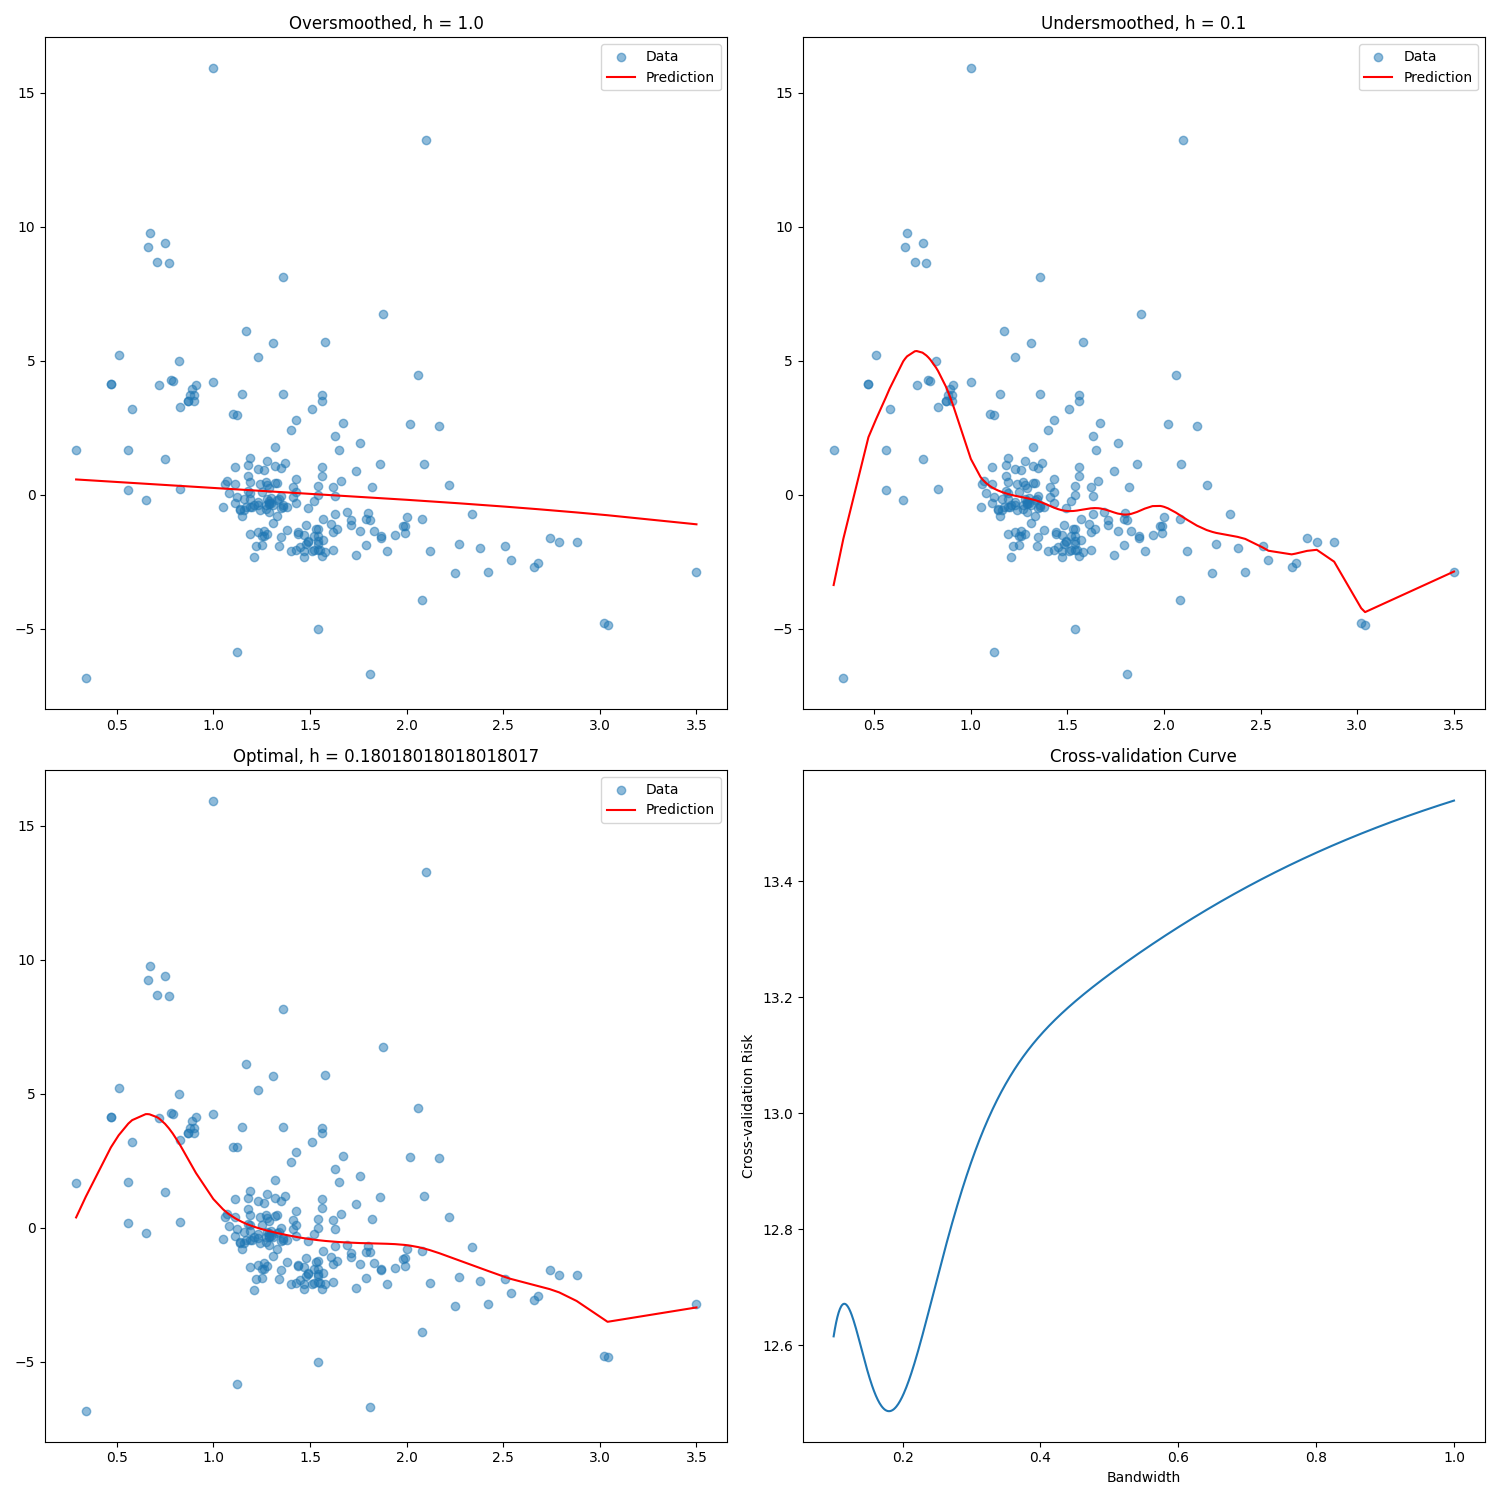
\includegraphics[width=0.5\textwidth]{../images/4/gaussian_kernel_regression.png}
	\caption{Oversmoothed, undersmoothed, optimal and cross validation curve of gaussian kernel}
\end{figure}

\begin{figure}[H]
	\centering
	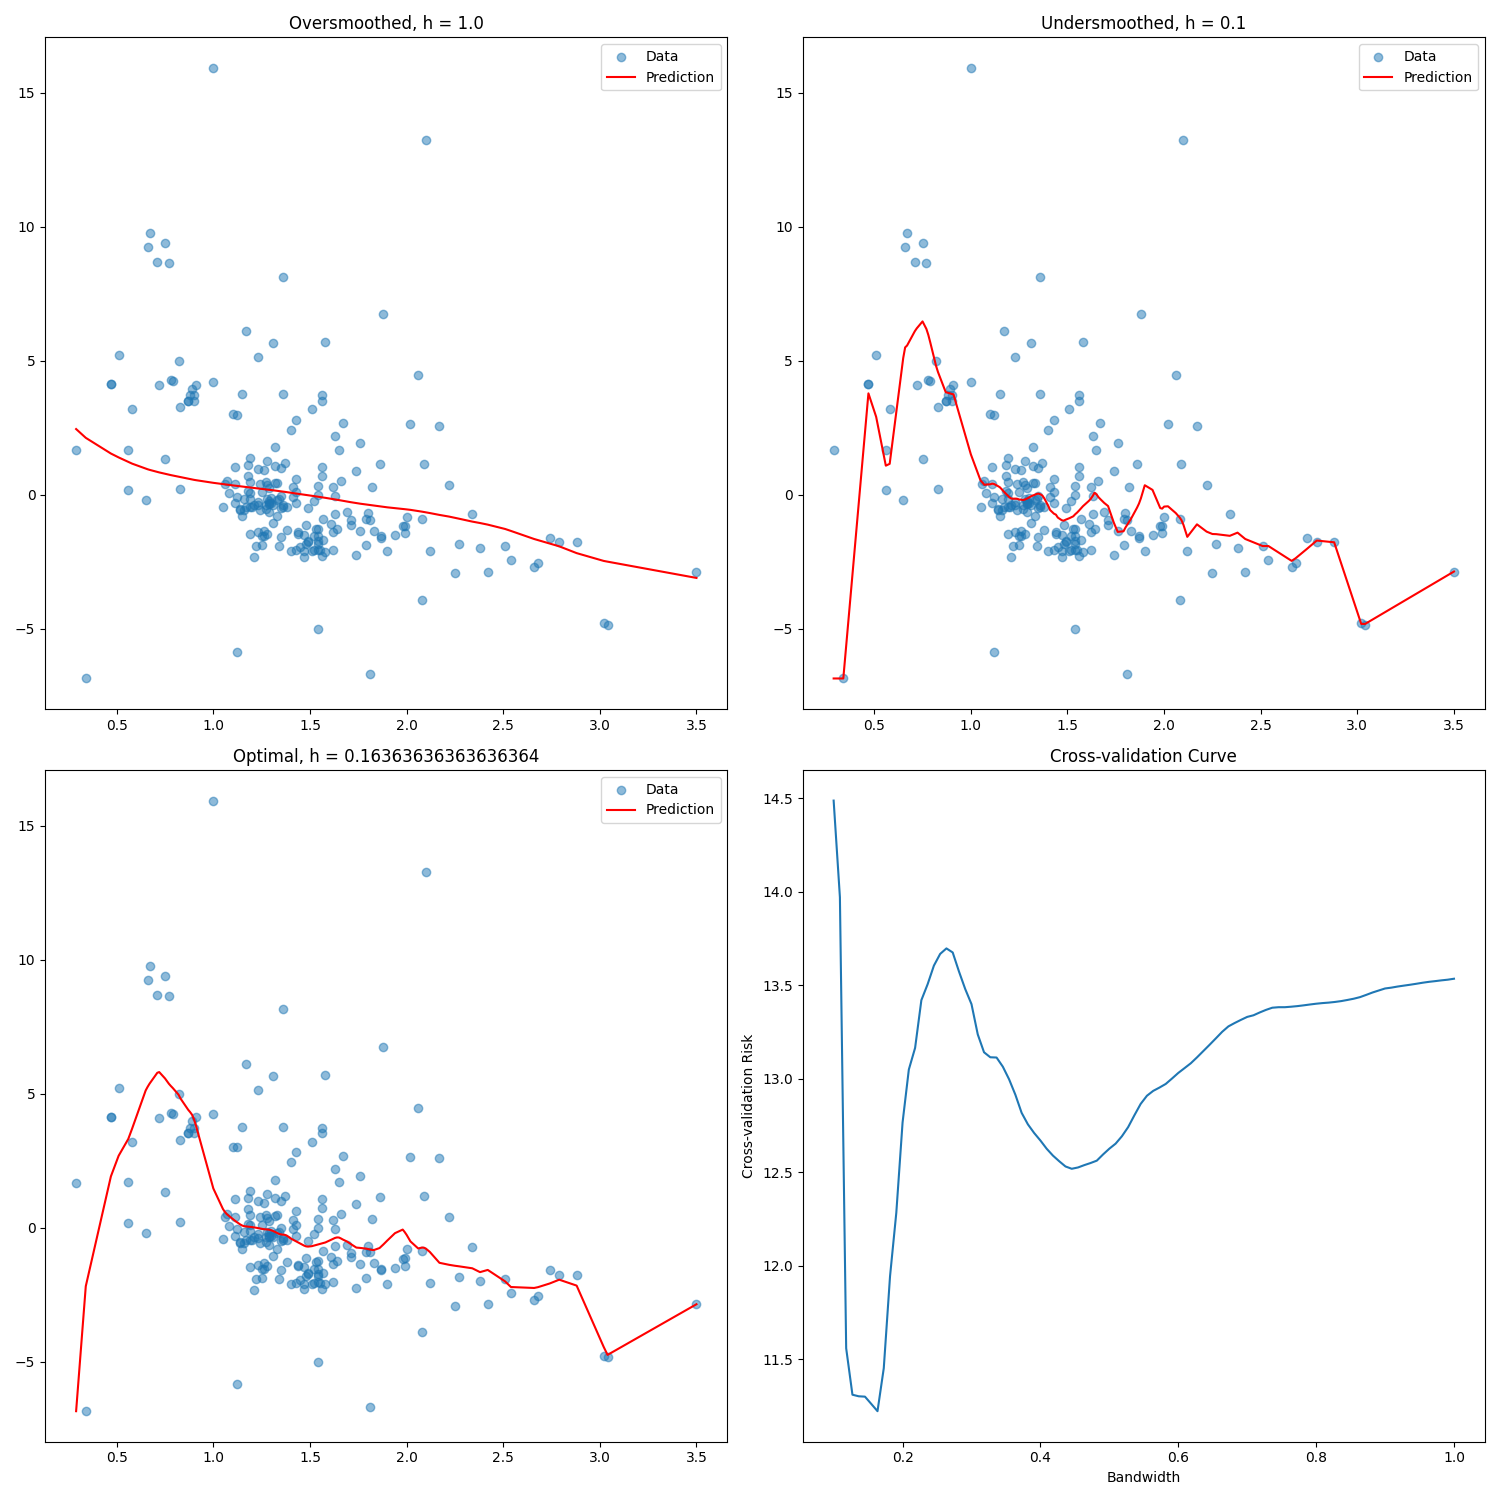
\includegraphics[width=0.5\textwidth]{../images/4/epanechnikov_kernel_regression.png}
	\caption{Oversmoothed, undersmoothed, optimal and cross validation curve of epanechnikov kernel}
\end{figure}

\begin{solution}

	\tcbsubtitle{Task A}

	Given, PDF of GMM variable $X$ is $f_X = \sum_{i=1}^K p_iP[X_i=x]$. Let
	it's CDF be $F_X$. Then $F_X(x)$ is given by

	\begin{align}
		F_X(x) & = P[X\leq x]                                    \\
		       & = \int_{-\infty}^{x} f_X(t)dt                   \\
		       & = \int_{-\infty}^{x} \sum_{i=1}^K p_iP[X_i=t]dt \\
		       & = \sum_{i=1}^K p_i\int_{-\infty}^{x} P[X_i=t]dt \\
		       & = \sum_{i=1}^K p_iP[X_i\leq x]                  \\
		       & = \sum_{i=1}^K p_iF_{X_i}(x)
	\end{align}
	Where $F_{X_i}(x) = P[X_i\leq x]$ is CDF of $X_i$.

	Now, let CDF of output of the given algorithm be
	$F_\A(x) = P[\A\leq x]$. Since the events that we choose $\A$ to be
	from the distribution $i$ (say $E_i$) are disjoint for $i=1,\dots,k$.
	\begin{align}
		F_\A(x) & = P[\A\leq x]                                \\
		        & = \sum_{i=1}^K P[E_i]\cdot P[\A\leq x | E_i] \\
		        & = \sum_{i=1}^K p_iF_{X_i}(x)                 \\
		        & = F_X(x)
	\end{align}

	We know that PDF of a random variable $X$ with CDF $F_X(x)$ is
	$\frac{\partial F_X}{\partial x}$. Thus,
	\begin{align}
		f_\A(x) & = \frac{\partial F_\A}{\partial x} \\
		        & = \frac{\partial F_X}{\partial x}  \\
		        & = f_X
	\end{align}

	Since $x$ was arbitrary, for every $u\in\mathbb{R}$, $f_\A(u) =
		f_X(u)$. i.e the algorithm indeed samples from the GMM variable's
	distribution.


	\tcbsubtitle{Task B}

	Since
	\begin{align}
		\E[X] & = \int_{-\infty}^{\infty} t\cdot P[X=t]dt                    \\
		      & = \int_{-\infty}^{\infty} t\cdot \sum_{i=1}^K p_iP[X_i=t] dt \\
		      & = \sum_{i=1}^K p_i \int_{-\infty}^{\infty} P[X_i = t] dt     \\
		      & = \sum_{i=1}^K p_i \E[X_i]                                   \\
		      & = \sum_{i=1}^K p_i\mu_i
	\end{align}

	Let $\mu = \E[X]$.
	\begin{align}
		\Var[X] & = \int_{-\infty}^{\infty} (t-\mu)^2 P[X=t] dt                    \\
		        & = \int_{-\infty}^{\infty} (t-\mu)^2 \sum_{i=1}^K p_iP[X_i=t] dt  \\
		        & = \sum_{i=1}^K p_i \int_{-\infty}^{\infty} (t-\mu)^2 P[X_i=t] dt \\
		        & = \sum_{i=1}^K p_i \Var[X_i]                                     \\
		        & = \sum_{i=1}^K p_i\sigma_i^2
	\end{align}

	Let $\sigma^2 = \Var[X]$.
	\begin{align}
		\MGF_X(t) & = \int_{-\infty}^{\infty} e^{tX}P[X=x]dx                     \\
		          & = \int_{-\infty}^{\infty} e^{tX} \sum_{i=1}^K p_iP[X_i=x] dx \\
		          & = \sum_{i=1}^K p_i \int_{-\infty}^{\infty} e^{tX}P[X_i=x] dx \\
		          & = \sum_{i=1}^K p_i\MGF_{X_i}(t)                              \\
		          & = \sum_{i=1}^K p_i e^{t\mu_i + \frac{1}{2}t^2\sigma_i^2}
	\end{align}

	\tcbsubtitle{Task C}
	Given $Z=\sum_{i=1}^Kp_iX_i$, where $X_i\sim\N(\mu_i,\sigma_i^2)$

	\begin{align}
		\E[Z] & = \E\left[\sum_{i=1}^Kp_iX_i\right] \\
		      & = \sum_{i=1}^Kp_i\E[X_i]            \\
		      & = \sum_{i=1}^Kp_i\mu_i
	\end{align}

	% \begin{align}
	% 	\Var[Z] & = \Var[\sum_{i=1}^Kp_iX_i]    \\
	% 	        & = \sum_{i=1}^Kp_i^2\Var[X_i]  \\
	% 	        & = \sum_{i=1}^Kp_i^2\sigma_i^2
	% \end{align}
\end{solution}

% Start writing your answer from here, if you want to use new packages/change something do it in main.tex
\begin{que}
	Suppose that you have computed the mean, median and standard deviation of a
	set of $n$ numbers stored in array $A$ where $n$ is very large. Now, you decide
	to add another number to $A$. Write a python function to update the
	previously computed mean, another python function to update the previously
	computed median, and yet another python function to update the previously
	computed standard deviation. Note that you are not allowed to simply
	recompute the mean, median or standard deviation by looping through all the
	data. You may need to derive formulae for this. Include the formulae and
	their derivation in your report. Note that your python functions should be
	of the following form:

	\begin{verbatim}
	function newMean = UpdateMean(OldMean, NewDataValue, n, A),
	function newMedian = UpdateMedian(OldMedian, NewDataValue, n, A),
	function newStd = UpdateStd(OldMean, OldStd, NewMean, NewDataValue, n, A).
	\end{verbatim}

	Also explain, how would you update the histogram of $A$, if you received
	a new value to be added to $A$? (Only explain, no need to write code.)
	Please specify clearly if you are making any assumptions.
	\hspace*{\fill}[10 marks]
\end{que}

\begin{tcolorbox}
	\begin{sol}
		% Add your solution here
	\end{sol}
\end{tcolorbox}

\begin{que}
	Read about the following plots:
	\begin{enumerate}
		{\color{red}
		\item Violin Plot
		\item Pareto Chart
		\item Coxcomb Chart
		\item Waterfall Plot
		      }
	\end{enumerate}
	Describe the uses of these plots. Take some sample data and generate one example plot
	for each of them.

	\hspace*{\fill} [8 marks]
\end{que}

\begin{tcolorbox}[breakable]
	\begin{sol}
		Here are the descriptions and usages of the given plots along with their examples:
		\begin{enumerate}
			\item \textbf{Violin plot:} It's a hybrid of box plot and kernel density plot.
			      A box plot represents data in a linear fashion. It's made of a straight line
			      from lowest value to highest value along with a box from first to third
			      quartiles, marking all the quartiles of the dataset. Here's an example:
			      \begin{figure}[H]
				      \centering
				      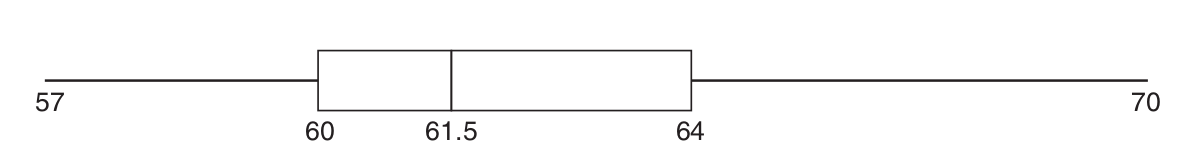
\includegraphics[width=0.5\textwidth]{box_plot}
				      \caption{Box plot}
				      \label{fig:box}
			      \end{figure}
			      A kernel density plot represents the density/frequency of data points. It's
			      similar to a histogram, but smooth. In a violin graph, this is kept vertical,
			      with two mirror images of it reflected along y-axis. This is useful in the
			      sense that we can look into both centrel tendencies of the data (like mean,
			      median etc.) but also how the data is distributed. Both at once. We can
			      visualise the following data which I've taking from (*) containing the average
			      number of hours a person studies given the number of courses taken
			      \begin{figure}[H]
				      \centering
				      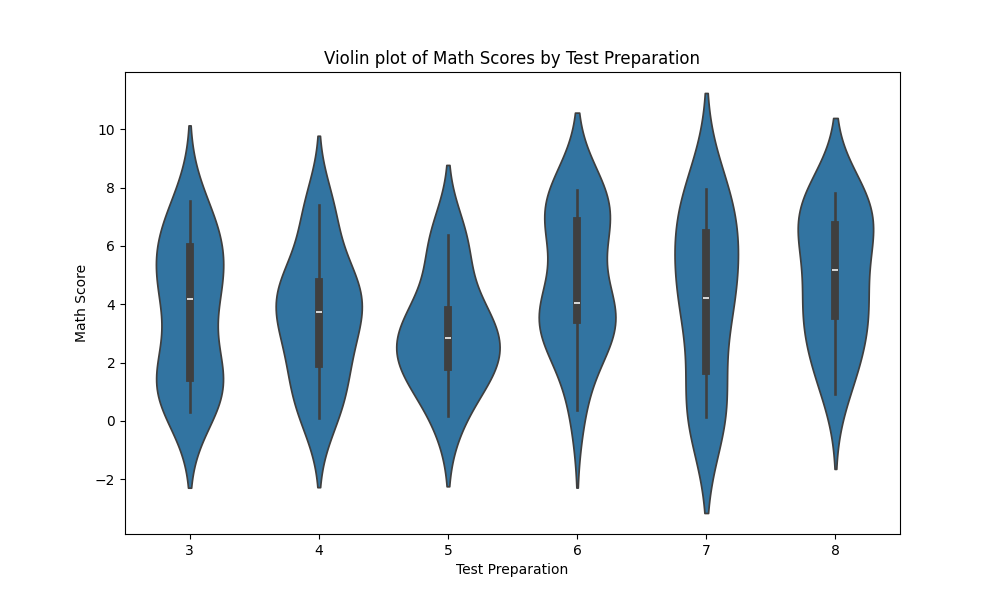
\includegraphics[width=0.7\textwidth]{violin-plot}
				      \caption{Violin Plot}
				      \label{fig:violin}
			      \end{figure}
			      As mentioned before, a violing plot can show both statistical summary along
			      with distribution, which a normal plot can't. Here, the gray line represents
			      the box plot component of it. And the plot you get by rotating it by $90^\circ$
			      is the distribution plot.
			  \item \textbf{Pareto Chart:} 
		\end{enumerate}
	\end{sol}
\end{tcolorbox}

% Start writing your answer from here, if you want to use new packages/change something do it in main.tex
\begin{que}
	Download the image of Monalisa from here. Read the image using matplotlib (example). Write a
piece of python code to shift the image along the X direction by tx pixels where tx is an integer
ranging from -10 to +10 (so, in total you need to do this for 20 values). While doing so, assign
a value of 0 to unoccupied pixels. For each shift, compute the correlation coefficient between the
original image and its shifted version. Make a plot of correlation coefficients across the shift values.
Also, generate a normalized histogram for the original image. You might need to refer to section
3.3 from this book. You are not allowed to use any inbuilt function for generating the histogram.
If you are using any other libraries, then please mention about them in the pdf.

	\hspace*{\fill} [8 marks]
\end{que}

\begin{tcolorbox}
    \begin{sol}        
        The image of Mona Lisa was read using the \texttt{matplotlib} library. The image was then shifted horizontally by \texttt{tx} pixels for each value of \texttt{tx} in the range of -10 to +10. The shifting operation was implemented manually, ensuring that unoccupied pixels were assigned a value of 0.
        
        A custom function \texttt{shiftimg} was created to handle the shifting process:
        \begin{itemize}
            \item If \texttt{tx > 0}, pixels were shifted rightwards by \texttt{tx} units.
            \item If \texttt{tx < 0}, pixels were shifted leftwards by \texttt{tx} units.
            \item If \texttt{tx = 0}, the function returned the original image.
        \end{itemize}
        
        For each shifted image, the correlation coefficient between the original and shifted image was calculated. This coefficient quantifies the linear relationship between the two images, with values ranging from -1 to 1, where 1 indicates a perfect positive correlation, -1 indicates a perfect negative correlation, and 0 indicates no correlation.
        A normalized histogram of the original image was generated by calculating the frequency of each pixel intensity and then normalizing the values. This was done manually without using any inbuilt histogram function.
        \newpage
        The correlation coefficients for the different shift values were plotted to observe the relationship between the magnitude of the shift and the correlation with the original image.
        
        \begin{figure}[H]
            \centering
            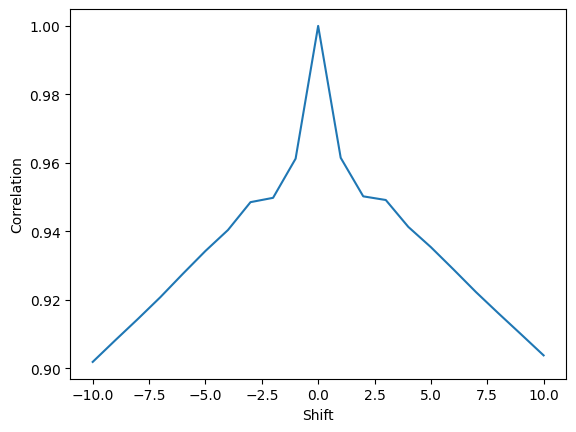
\includegraphics[width=0.8\textwidth]{correlation_plot.png}
            \caption{Correlation Coefficient vs Shift Values}
            \label{fig:corr_plot}
        \end{figure}
        
        
        As observed in Figure \ref{fig:corr_plot}, the correlation decreases as the shift increases in either direction. This is expected as the more the image is shifted, the less it resembles the original, resulting in lower correlation values.
        
        The normalized histogram of the original image was also plotted to visualize the distribution of pixel intensities.
        
        \begin{figure}[H]
            \centering
            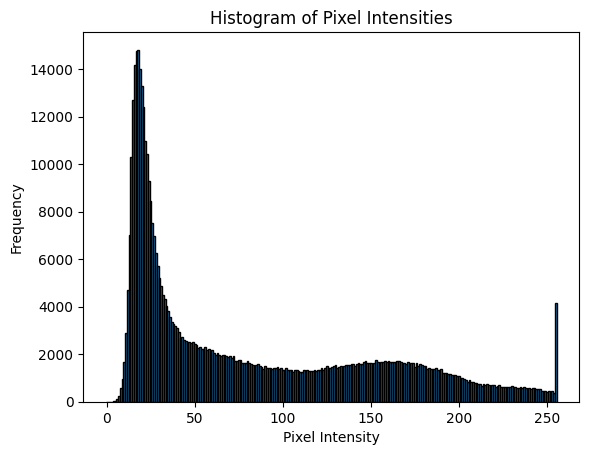
\includegraphics[width=0.8\textwidth]{red_pixel_intensity.png}
            \caption{Normalized Histogram of the Original Image}
            \label{fig:hist_plot}
        \end{figure}
        
        The histogram in Figure \ref{fig:hist_plot} shows the frequency of occurrence of each pixel intensity, normalized over the total number of pixels.
              
        

        
    \end{sol}
\end{tcolorbox}
\end{document}
